%------------------------------------------------------------------
%
% Vorlage für Abschlussarbeiten an der Technischen Hochschule Ingolstadt
% Bachelorarbeit/Masterarbeit
%
% Angepasst auf Seminararbeit
%
% V1 05.12.2011		Dr. Paul Spannaus
% V2 07.07.2012		Dr. Paul Spannaus
% V3 10.03.2013		Dr. Paul Spannaus
% V4 28.01.2014		Dr. Paul Spannaus
% V5 31.10.2014 		Dominik Schlecht
% 	
% -----------------------------------------------------------------
% -----------------------------------------------------------------

% Dokumentenklasse
\documentclass[a4paper,11pt,DIV=11,twoside]{scrreprt} % 

% Packages
%Datum und Uhrzeit
\usepackage{datetime}

%Encoding
\usepackage[utf8]{inputenc}
\usepackage{lmodern}

%Graphikpakete
\usepackage{graphicx}
\usepackage{xcolor}
\usepackage{tikz}
\usetikzlibrary{arrows, snakes, backgrounds}
\usepackage{wrapfig}

% Farben der THI
\definecolor{THIblue}{rgb}{0.0078,0.1176,0.4705}

\usepackage[ngerman]{babel}

%Zitierumgebung
%\usepackage{cite}% Zitieren
\usepackage[backend=biber,]{biblatex}
%\usepackage{bibgerm}% Literatur in Deutscher DIN
\usepackage[babel,german=quotes]{csquotes}

%%-------------Silbentrennung--------------------------------------
\hyphenation{}

%%-------------Index-----------------------------------------------
%\makeindex

%------------------------------------------------------------------
% Angabe der zu verwendenden Dateien, sodass nur z.B. das aktuelle 
% Dokument compiliert wird; den Rest mit % auskommentieren
\includeonly{
    chapter/Intro,
    chapter/Dungeon,
    chapter/Tweety_bird,
    chapter/ATM_Machine,
    chapter/Text_File_Store,
    chapter/Setup
}

%-----------------------------------------------------------------
%---------------Dokumentenbeginn----------------------------------
%-----------------------------------------------------------------
\begin{document}
	%\pagenumbering{roman} % Nummerierung
%---------------Hauptteil-----------------------------------------
	%\pagenumbering{arabic} 	% Neunummerierung des Hauptteils
	%\setcounter{page}{1}	% Wieder bei 1 Anfangen
	
	%intro
	\chapter{Intro}
Der iCTF (international Capture The Flag) wird jährlich von der University of California, Santa Barbara veranstaltet und ist der größten Hackerwettbewerbe dieser Art. 
Der iCTF integriert Angriff und Verteidigung zugleich. Die Teilnehmer müssen gleichzeitig Flaggen von fremden Servicen klauen, sowie ihre eigenen Service patchen um diese unangreifbar zu machen. 
Dieses Jahr fand der Wettbewerb am 04.12. statt und ca. 40 Teams nahmen daran Teil. Dabei belegte unser Team (in23canation) den 22. Platz. Die Dauer des Wettbewerbs wurde mit 24 Stunden angekündigt jedoch kurz vor dem iCTF auf 8 Stunden reduziert. 
Die Stimmung beim Wettbewerb war durchgehend positiv und insgesamt war der CTF ein großer Erfolg. Durch etwas Werbung vorab war es möglich eine große Teilnehmerzahl aus allen Semestern zu begeistern sich unserer Gruppe anzuschließen. Schon bei den zwei vorangehenden Informationsveranstaltungen waren ungefähr 60 Studenten anwesend. Beim iCTF selber waren rund 25 Teilnehmer aktiv dabei. 
	
	%setup
		\section{Network-Setup}
	The setup of the iCTF 2015 is shown in the graphic \ref{img:setup}. The Router has a private VPN running, tunneling all traffic through the THI-Network. Also the Router creates 2 sub-networks. The "bad network" (shown in red) holds the iCTF-Router and vulnerable VM, as well as some attacker PCs, which will run the exploits against other teams. In the "good network" (shown in green) are the participants, who have a local copy of the vulnerable Image and develop patches and exploit. It's to mention, that the router has ip-tables-rules specified, so the "bad network" can not communicate with the "good network". Also, the Attacker-PCs have to route their traffic through the CTF-Router. This should be solved differently in the upcoming CTFs, since the separation of the 2 networks needed a lot of time to be configured.
	\begin{figure}
		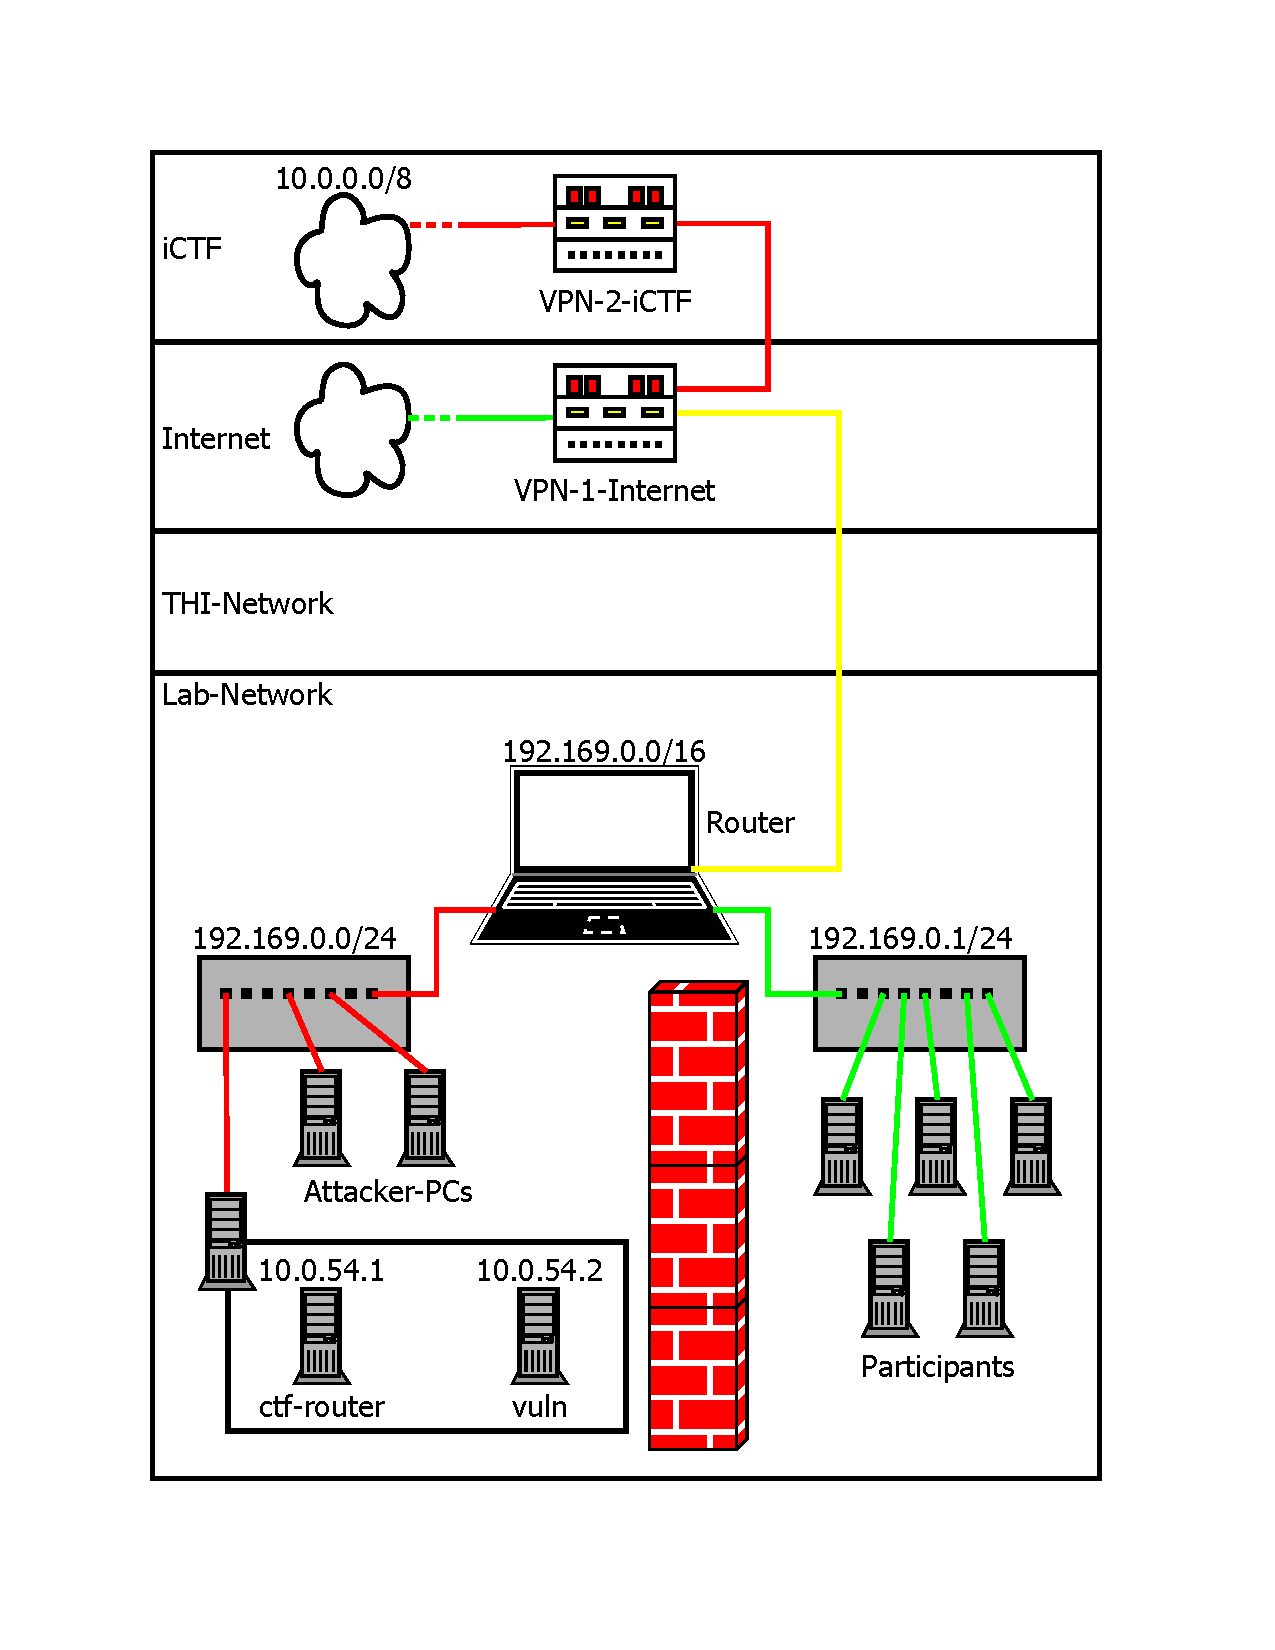
\includegraphics[width=\textwidth]{images/setup.pdf}
		\caption{Network-Setup iCTF 2015}
	\end{figure}
	%Dungeon Service
	\label{img:setup}
	
	%Dungeon Service
	\chapter{Dungeon}


\section{Aufbau und Configuration}


\section{Services: Dungeon}
The Dungeon service was a consoleservice which presented a litte game. The player needs to run through the dungeon to finally kill a dragon in the end. To do this, two items are needed. Firstly a golden sabre and second a magic shield. If either of the items is missing the player will die to the dragon.
To get the sabre the player needs to find a secret room and in there has to get the name of an airplane picture right. If he does he will get the sabre. 
Now the player will get in a room with a dwarf. He says if you get the number i guess you will get my shield. But the number he has is random generated and nearly impossible to get right. Also if you get the number right he will tell you that he gives you the shield but the variable HAVE\_SHIELD will not change. To achive the shield the player has to go to a room with a gnome which asks the player's name and then says Hi! playername. In this function there is an adress returned with the variable HAVE\_SHIELD. So the player need to type in anycharacter than \%n so that the adress will be overwritten with 0x1.
If the player encounters the dragon with both items he can slay the dragon with the command "'kill dragon"'. After that he will be asked what his name is. Here comes the tricky part. With a Bufferoverflow it is possible to alter the return adress so that the function will jump to the secret treasure room where the flag can be optained. To do this the player have to type 88 random characters followed by 0xDEADBEEF in ASCII than 8 random characters again and then the adress to the storage room. The 0xDEADBEEF is needed because a value is checked for change. If you overwrite it with the bufferoverflow the service will disconnect the player. Both 0xDEADBEEF and the return adress have to be turned because little Endian is used. 


%Der Dungeon Service war ein Consolenservice der ein Spiel darstellt. der Spieler muss dabei durch ein Dungeon laufen und am Ende einen Drachen töten. Um dies zu bewerkstelligen werden 2 Gegenstände gebraucht. Ein goldener Säbel und ein magisches Schild. 
%Um den Säbel zu bekommen muss zuerst ein geheimer Raum gefunden werden in dem der Namen eines Flugzeuges anhand eines Abbilds erraten werden muss. Wird richtig geraten erhält der Spieler den Säbel. 
%Des weiteren gibt es einen Raum, bei dem ein Zwerg sein Schild abgibt, wenn du seine Nummer errätst. Dies ist jedoch fast unmöglich da die Nummer zufällig bestimmt wird. Des weiteren bekommt man den Schild ebenfalls nicht wenn man die Nummer errät. 
%Um diesen nun zu bekommen muss in einem anderen Raum bei einem Gnom der nach den Spielernamen fragt den Speicher überschreiben. Die Funktion übergibt die Adresse der Variable HAVE\_SHIELD und wenn man ein beliebiges Zeichen und dann \%n eingibt, wird auf der Adresse HAVE\_SCHIELD eine 1 eingetragen. 
%Wenn der Spieler nun beim Drachen ist, stirbt er nicht wie sonst, sondern kann den Drachen mit dem command  "'kill dragon"' töten. 
%Im Anschluss daran wird er Spieler erneut nach seinem Namen gefragt. Nun kann man mithilfe eines Bufferoverflows die Rücksprungadresse der Funktion so ändern, dass der Spieler im Secret Storage Room landet. Dort wird die Flagge ausgegeben, wenn die ID angegeben wird. Eine Hürde beim Bufferoverflow ist jedoch, dass auf eine Variable geprüft wird und wenn die überschrieben wird, wird der Nutzer vom Service getrennt. Um dies zu verhindern muss genau ab der 88. Stelle 0xDEADBEEF in ASCII mitübergeben werden. Danach noch 4 Zufallszeichen und dann die Rücksprungadressse. 0xDEADBEEF sowie die Rücksprungadresse müssen umgedreht werden, das litte Endian verwendet wird.
	
	%Tweety Bird Service
	\chapter{Tweety\_bird}

The service tweety\_bird was a console service, which saved a secret in a file and stored a password for it in another file. This was done by selecting write("'X"') and entering "'\textless filename\textgreater \textless secret\textgreater \textless password\textgreater"'. 

The secret could be retrieved by selecting read("'R"') and entering "'\textless filename\textgreater \textless password\textgreater"'. The flag was the stored secret. After decompiling of the c-code and checking it, it was determined, that the password was written in an array of size 50. After that the password is compared with the right password or if its not empty. 

In case of a bufferoverflow the compare value for empty will be overwritten and any password will be accepted. A first try with the Passwort 51 times "'A"' already was accepted and the secred was retrieved because the files were unencrypted. Closing the found security gap was not tried, because of the missing original c-code and time issues.
	
	%Text File Store
	\chapter{Text\_File\_Store}
If you open the site you can see a form where you can login with a username and password or you can enter a short message you want to store.
After storing some text you get the username and the password to look for that text later. The username and the password are calculated at runtime of the service. 

Every parameter of the service are passed in the URL via GET. In the viewFile.php file you can find a parameter called "file". This parameter is used to access a file in the directory where all textfiles are stored. 

But if you modify this parameter you can read the content of the access.log file without any verification. 
In this file you can see every connection to this service. At last you have to filter for the flags and read them. 
Also it is possible to inject a command with an adjusted url call. It generates a file on the server with the filenames in the service-directory. With this information it is possible to open the files containing the flags. 
	
	%ATM Machine
	\chapter{ATM\_Machine}

The ATM\_Machine Service is a bank automate service in which the user has three options. It is possible to create an account with a ping, to check the balance of an account and to withdraw money from an account. If the user tries to withdraw more money than he has, the service will close the connection. 

At First the ATM.jar File was Decompiled using the JAD-Decompiler. After that a simple string concatenation was found which leadd to the possibility of a SQL-Injection. After that the structure of the Database was analized and with the SQLite editor test injection were tried. 

After some testing the solution was to connect to the service, than choose option 1 to check the account Balance. After that the service ask for an account number here the user can type in any char. Now the service needs the pin and here we can use the SQL injection.
The statment we need ist UNION ALL SELECT acnum, cash, password FROM login WHERE acnum = ''"' + self.flagID. Now the service returns the password for the falgID which is the flag itself.

For the statement we need the UNION ALL SELECT to unite the existing statment result with the injected one. We only need the password from the database but because the service only returns the thid collumn we need two previous ones. Thats why acnum, cash, password was used with password in the third collumn. "'FROM login WHERE acnum = ''"' + self.flagID"' was used to read the password from the correct table using the given account number which was the flagID given from the provider.



%ATM Machine Writeup
%=====================
%(Simon Varga, Markus Monz)
%
%1. Decompile Java service [ATM.class] using JAD-Decompiler
%2. See simple string concatenation instead of prepared statement [line 29]
%3. Watch SQLite database structure [see <pathToService>/rw/database.db]
%4. Use SQLite editor to execute test injection statements [solution see exploit]
%
%
%Description of Exploit
%=====================
%1. $> Connect to service with nc on port 20051
%2. Service asks to choose banking operation
%3. $> Choose option "1" [Check account balance]
%4. Service asks for account number
%5. $> Give any character
%6. Service asks for pin [here comes the magic, inject SQL statement]
%7. $> "1' UNION ALL SELECT acnum, cash, password FROM login WHERE acnum = '" + self.flagID
%8. Service returns the password, which is the flag, related to the given account number
%
%Exploit Components
%=====================
%    "1'" - close the existing statement
%    "UNION ALL SELECT" - unite the existing statement result with the injected one
%    "acnum, cash, password" - put password in the third column, because the service only returns the third column
%    "FROM login WHERE acnum = '" + self.flagID" - read the password from the correct table using the given account number
%
%Exploit [python]
%=====================
%    s.send('1\n')
%    s.send('blub\n')
%    s.send("1' UNION ALL SELECT acnum, cash, password FROM login WHERE acnum = '" + self.flagID)
%    flag = s.recv(512)
%    p = re.compile('Your Balance is: (FLG.{13})')
%    m = p.match(flag)
%    flag = m.group(1)
	
%---------------Anhang-------------------------------------------
	%
%------------------------------------------------------------------------
% Anhänge
\appendix
\chapter{Appendix}
\section{Quellcode}
\section{Ergänzende Grafiken}
\section{Quellcode Grafiken}
 % Anhang
	%\newpage
	%\printbibliography % Literaturliste
\end{document}
%-----------------------------------------------------------------
%---------------Dokumentenende------------------------------------
%-----------------------------------------------------------------
